\documentclass[11pt]{article}

\usepackage{maiacustom}

\begin{document}

\psettitle{Banco de questões de astronomia}

Estas questões foram produzidas/selecionadas cuidadosamente com o objetivo de preparar os estudantes para o processo seletivo de astronomia no Brasil. Algumas questões não são de autoria própria e estão devidamente sinalizadas por () antes do enunciado. O template do banco de questões é o mesmo do Professor \text{Kevin Zhou}. Seu trabalho é valioso, e diversas ideias desta lista podem ser encontradas em seus Handouts.

% \begin{psidea}{Título da Ideia}{}
% Ideia
% \end{psidea}

% \begin{psexample}{Título do Exemplo}{}
% Exemplo
% \end{psexample}

% \begin{pssolution*}{}{}
% Solução
% \end{pssolution*}

% \begin{psremark*}{Título da Observação}{}
% Observação
% \end{psremark*} 

\section{Mecânica Celeste}
\pts{5}    
\begin{pproblem}
    Iaum e Sevla, dois físicos renomados, pretendem lançar uma sonda espacial para explorar os limites da física newtoniana e as correções relativísticas necessárias nas proximidades de um buraco negro. Eles precisam da sua ajuda para estudar o \textit{Potencial Efetivo} de tal corpo.
    \begin{enumerate}[label=\textbf{\alph*)}]
        \item A energia de um corpo de massa \(m\) orbitando um corpo massivo de massa \(M\) pode ser escrita como:
             \[
             \frac{m\dot r ^2}{2} + V_{eff}(r)
             \]
             Onde \(\dot r\) é a velocidade radial do corpo. Encontre \(V_{eff}(r)\) em função de \(G\), \(M\), \(L\), \(m\) e \(r\).

        \item Segundo a física newtoniana, qual é o menor raio no qual é possível um corpo possuir uma órbita circular em torno de um buraco negro?
    
        \item Qual é a frequência de pequenas oscilações radiais, \(\omega_r\), em torno desse raio?

        O potencial gravitacional próximo a esses corpos precisa sofrer uma correção relativística e tem a forma:
        \[
        V(r) = -\frac{GMm}{r} - \frac{GML^2}{mc^2r^3}
        \]

        \item Explique por que essa correção permite que uma partícula caia no centro de um buraco negro, \(r=0\), e por que isso é impossível na física newtoniana.
        
        \item Qual é o menor valor de \(L\) para que uma partícula possa orbitar o buraco negro em uma órbita circular? Qual é o valor do raio nessa condição?
        
        \item Assumindo \( \lim_{L \to \infty}\), encontre a menor distância que uma partícula em órbita aberta pode se aproximar de um buraco negro.  
    \end{enumerate}
    
\end{pproblem}

\pts{3}
\begin{pproblem} Um ponto importante no estudo de órbitas é o que acontece quando o potencial segue algo incomum. O objetivo desta questão é estudar esse fenômeno. Considere o momento angular \(L\) e a massa do corpo \(m\).
    \begin{alternativas}
        \item Para uma órbita geral, que possui um potencial \(V(r)\) na forma \(\psi r^k\), encontre o valor \(r_0\) de uma órbita circular para esse potencial.
        
        \item Encontre a frequência de pequenas oscilações, \(\omega_r\), em torno desse raio. 
        
        \item Seja \(\omega_\theta\) a frequência angular da órbita, encontre o valor da razão \(\frac{\omega_r}{\omega_\theta}\). Uma órbita só pode ser fechada se essa razão for um número inteiro. Por quê? Encontre valores de \(k\) para que a órbita seja fechada.
         
    \end{alternativas} 

    
\end{pproblem}

\pts{4} %semana 114
\begin{pproblem}
    O Hodógrafo é uma das maneiras menos conhecidas de resolver questões de mecânica celeste. Ao usar esse mecanismo, é possível resolver questões complexas (envolvendo encontrar parâmetros orbitais, parâmetros de velocidade e como minimizar a excentricidade de uma órbita, por exemplo). Apesar de o Hodógrafo possuir diversas utilidades, o objetivo deste exercício é provar o Teorema do Hodógrafo, que diz que, em órbitas fechadas, a velocidade forma um círculo no espaço vetorial. Vamos provar esse teorema de duas maneiras.
    \begin{align*}
    \textbf{Método 1)}
    \end{align*}
    \begin{enumerate}[label=\textbf{\Roman*.}]
        \item Partindo da Segunda Lei de Newton e da conservação do momento angular, encontre uma expressão para \(d\mathbf{v}/d\theta\). Deixe sua resposta em função do momento angular por unidade de massa, \(h\), e \(\mu\) = \(GM\). 
        \item Onde o centro desse círculo está localizado? Considerando o corpo central na origem do sistema, determine uma expressão para a distância entre o corpo central e o centro do Hodógrafo. 
    \end{enumerate}
    
    \begin{align*}
        \textbf{Método 2)}
    \end{align*}
    O método 2 utiliza noções de cálculo mais avançadas e parte da conservação do \textit{vetor de Laplace-Runge-Lenz}, \(\mathbf{A}\).
    \begin{enumerate}[label=\textbf{\Roman*.}]
        \item O vetor \(\mathbf{A}\) é dado pela expressão:
        \[
        \mathbf{A} = \mathbf{p}\times \mathbf{L} - GMm^2\mathbf{\hat{r}}
        \]
        O primeiro passo para a demonstração é provar que \(\mathbf{A}\) é constante. Para isso, derive o mesmo em relação ao tempo e tire suas próprias conclusões.
        \item Como o vetor \(\mathbf{L}\) é constante, \(\mathbf{A}\times\mathbf{L}\) também é uma constante. Utilizando a identidade vetorial \(\mathbf{A}\times(\mathbf{B}\times\mathbf{C}) = \mathbf{B}(\mathbf{A}\cdot\mathbf{C}) - \mathbf{C}(\mathbf{A}\cdot\mathbf{B}) \), prove que \(\mathbf{v}\) forma um círculo no espaço vetorial.    
    \end{enumerate}
    
\end{pproblem}

\pts{2} %problemas da semana 114
\begin{pproblem} Um dos fenômenos mais fascinantes do sistema solar são as estrelas de nêutrons. Esses são corpos muito pequenos, super densos e que giram muito rápido. Nesta questão, vamos fazer um modelo teórico para essas estrelas.
    \begin{enumerate}[label=\textbf{\alph*)}]
        \item O Pulsar da Vela, uma estrela de nêutrons localizada na constelação da Vela, possui uma frequência de \(11 \text{Hz}\), ou seja, ela gira em torno de si mesma \(11\) vezes por segundo, raio equatorial \(R_e = 9,6\text{ km}\) e massa \(M = 1,88M_\odot\). Sabendo disso, calcule a razão entre seu raio equatorial e seu raio polar.
        \item Qual é o menor período de rotação que o Pulsar da Vela pode ter para que ele não se despedace?
        \item Atualmente, a taxa de variação do período do Pulsar da Vela é \(\frac{\Delta P}{\Delta t} = 1,25 \cdot 10^{-13}\text{s/s}\). Isso faz com que o Pulsar libere uma quantidade absurda de energia. A temperatura superficial do Pulsar é de \(T \sim 10^6\text{ K}\). Calcule a ordem de grandeza da razão entre a potência emitida pelo aumento do período e a potência emitida pela Lei de Stefan-Boltzmann.
    \end{enumerate}
    
\end{pproblem}

\pts{3}
\begin{pproblem} (Adaptado PPP) Geométrio, Paulinho e Hirata adoram chocolate. Certo dia, ambos estavam explorando uma galáxia quando se depararam com uma bola gigante de chocolate. Os três rapidamente começaram a comer a bola, primeiro fazendo uma linha reta do ponto \(P\) até o centro da bola em \(O\) (esquema \(1\)). Após isso, Hirata cai, colidindo no ponto \(O\), sem frear no caminho. Surpreendentemente, ele continua vivo e é resgatado por Geométrio e Paulinho. Após isso, famintos, eles continuam a comer a esfera gigante de chocolate e deixam um buraco esférico de diâmetro \(\overline{PO}\) (esquema \(2\)). Hirata é muito desastrado e acaba caindo de novo, partindo do ponto \(P\) e indo até \(O\) novamente.
    \begin{enumerate}[label=\textbf{\alph*)}]
        \item Encontre a razão entre as velocidades de impacto de Hirata nos casos \(1\) e \(2\).
        \item Encontre a razão entre os tempos de queda de Hirata nos casos \(1\) e \(2\).
    \end{enumerate}
    \begin{paracol}{2}
        \begin{figure}[h]
            \centering
            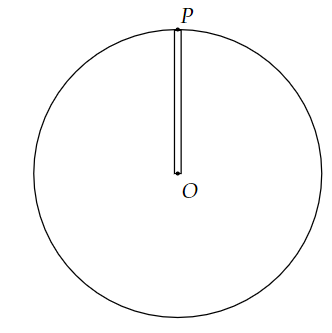
\includegraphics[width=0.31\textwidth]{imagens/q5(1).png}
            \caption{Esquema \(1\)}
        \end{figure}
        \switchcolumn
        \begin{figure}[h]
            \centering
            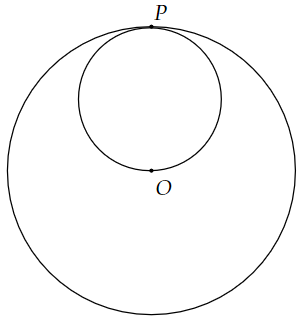
\includegraphics[width=0.3\textwidth]{imagens/q5(2).png}
            \caption{Esquema \(2\)}
        \end{figure}
    \end{paracol} 

   
\end{pproblem}

\pts{5}
\begin{pproblem} Calcular as velocidades de escape em certas situações pode ser mais complicado do que parece. Um exemplo disso é calcular a velocidade de lançamento que um foguete precisa ter para chegar a determinado local.
    \\
    \textbf{Dica:} Os problemas a seguir exigem que você pense cuidadosamente no referencial mais adequado. Não subestime a questão.
    \\
    \textbf{Dados:} Um corpo pode orbitar a superfície da Terra com velocidade \(v_0 = 7,9\text{ km/s}\), a velocidade orbital da Terra em torno do Sol é \(u_0 = 29,7\text{ km/s}\), e o raio da Terra é desprezível em relação à distância Terra-Sol. Considere também que, ao deixar o campo gravitacional da Terra, a distância entre a sonda e o Sol é a mesma distância entre a Terra e o Sol.
    \begin{enumerate}[label=\textbf{\alph*)}]
        \item Qual é a menor velocidade de lançamento que um foguete precisa ter para atingir o Sol, considerando que ele dê apenas um impulso? (Para conferir, \(v = 31,8\) km/s)
        \item Qual é a menor velocidade de lançamento que um foguete precisa ter para escapar do Sistema Solar? (Para conferir, \(v = 16,7\) km/s)
        \item Como a resposta do item \textbf{a)} muda se o foguete conseguir realizar um segundo impulso muito pequeno em algum ponto de sua órbita?
    \end{enumerate}

    
\end{pproblem}

\pts{3} % problemas da semana 115
\begin{pproblem} (Kevin Zhou) A equação dos foguetes é dada por:
    \[
    v = u\ln\left(\frac{M_0}{M}\right)
    \]
    Onde \(v\) é a velocidade do foguete, \(u\) a velocidade relativa com que o foguete ejeta combustível, \(M_0\) a massa inicial do foguete e \(M\) sua massa atual.
    \begin{enumerate}[label=\textbf{\alph*)}]
        \item Deduza a equação dos foguetes partindo da conservação do momento.
        \item Considerando \(u\) um valor fixo durante todo o percurso do foguete, qual deve ser o valor de \(u\) para que o foguete vá de \(0\) até \(v\) gastando o menor combustível possível? (Você precisará resolver numericamente para \(v/u\))
        \item Como a equação dos foguetes deve ser corrigida para uma região do espaço com um campo gravitacional, \(\mathbf{g}\), constante e apontando na direção contrária ao movimento do foguete? Considere \(\eta = dm/dt = \text{constante}\).
    \end{enumerate}

    
\end{pproblem}  

\pts{4}
\begin{pproblem} Um dos propelentes mais comuns em foguetes é uma mistura de hidrogênio líquido com oxigênio líquido. Quando começa a queimar, a seguinte reação química ocorre:
    \[
    2H_2 + O_2 \rightarrow 2H_2O
    \] 
    Para cada mol de hidrogênio, esta reação libera \(241,8 \text{ kJ}\) de energia. Ao longo da questão, suponha que toda essa energia seja utilizada para mover o foguete.
    \begin{enumerate}[label=\textbf{\alph*)}]
        \item Uma expedição espacial deseja ser feita de tal maneira que é necessário realizar uma transferência de Hohmann para lançar um foguete da Terra para Marte. Calcule a variação de velocidade total \(\Delta v\) necessária para realizar essa manobra.
        \item A partir do \(\Delta v\) calculado anteriormente, estime quantas toneladas de propelente devem ser utilizadas para realizar tal manobra para um foguete que ejeta propelente com velocidade \(u = 3,0\) km/s e carcaça com massa \(M = 140\cdot10^3\) kg.
    \end{enumerate}
    
\end{pproblem}

\pts{3} % problemas da semana 115
\begin{pproblem} Marisso estava estudando um sistema binário com inclinação \(i\). Ele conseguiu descobrir que o maior redshift vindo da estrela \(1\) era \(z_1\). Sabendo disso, ache uma expressão para a massa da estrela \(2\), \(m_2\), deixe sua resposta em função de \(z_1\), do período do binário \(P\), da inclinação \(i\), da razão entre as massas \(\lambda  = m_2/m_1\) e de constantes fundamentais. Considere as órbitas circulares.
    
\end{pproblem}

\pts{2}
\begin{pproblem} Qual é a razão entre \(a)\) as forças gravitacionais causadas pelo Sol e pela Lua na superfície da Terra? E \(b)\) das forças de maré causadas pelo mesmo?
    
\end{pproblem}

\pts{4}
\begin{pproblem} (Morin 7.7) Uma partícula de massa \(m\) viaja em uma órbita hiperbólica com uma massa \(M\) fixa em um dos focos. A velocidade no infinito é \(v_0\) e o parâmetro de impacto é \(b\).
    \begin{alternativas}
    \item Mostre que o ângulo de desvio da partícula é dado por:
    \[
    \phi = \pi-2\tan^{-1}(\gamma b)
    \]
    Onde \(\gamma \equiv v_0^2/GM\).
    \item Sendo \(d\sigma\) a seção transversal da partícula (medida quando a mesma se encontra no infinito) que é defletida em um ângulo sólido de tamanho \(d\Omega\). Mostre que:
    \[
    \frac{d\sigma}{d\Omega} = \frac{1}{4\gamma^2\sin^4(\phi/2)}
    \] 
    A título de curiosidade, essa quantidade é chamada de \textit{seção transversal diferencial}.
    \end{alternativas}

    
\end{pproblem}

\begin{psidea}{}{}
    Em certas questões, é válida a utilização de vetores. Um exemplo é a questão abaixo. Para facilitar, na parte de encontrar a inclinação da órbita, observe a seguinte imagem:

    \begin{figure}[H]
        \centering
        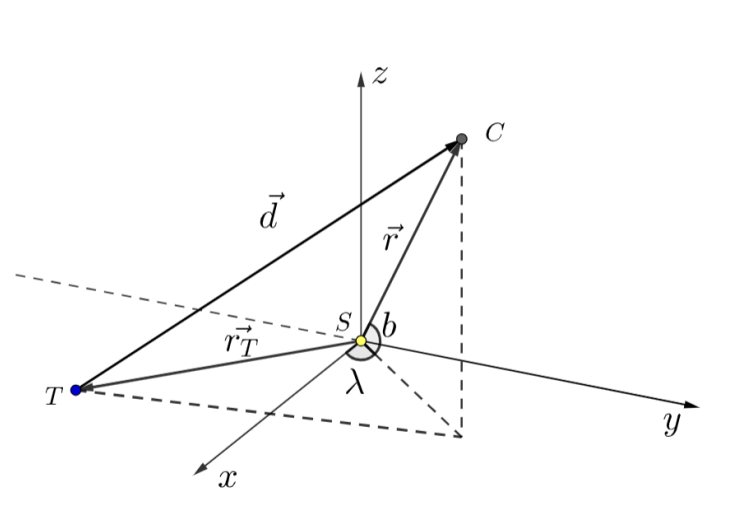
\includegraphics[width=0.7\linewidth]{imagens/vetores ecliptica.png}
        \caption{Vetores}
    \end{figure}

    Aqui, \(C\) representa um corpo, \(T\) a Terra e \(S\) o Sol. Os ângulos \(\lambda\) e \(b\) denotam, respectivamente, a longitude e a latitude eclíptica. \(\vec{r}\) é o vetor entre o Sol e o corpo, \(\vec{r}_T\) o vetor entre o Sol e a Terra, e \(\vec{d}\) o vetor entre a Terra e o corpo.
    Pela figura,

    \[\vec{r} = r(\cos b\cos\lambda \hat{x}+ \cos b \sin\lambda \hat{y} + \sin b \hat{z})\]

    \[\vec{r}_T = r_T(\cos(\omega_\oplus t)\hat{x}+\sin(\omega_\oplus t)\hat{y})\]

    Assim, \(\vec{d}=\vec{r}-\vec{r}_T\):

    \[
    \vec{d} = \big(r \cos b \cos \lambda - r_T \cos (\omega_\oplus t)\big) \hat{x} 
    + \big(r \cos b \sin \lambda - r_T \sin (\omega_\oplus t)\big) \hat{y} 
    + r \sin b \, \hat{z}
    \]

    Calculando o módulo do vetor \(\vec{d}\), obtemos que:

    \[
    d = |\vec{d}| = \sqrt{r_T^2 + r^2 - 2 r_T r \cos b \cos (\lambda - \omega_\oplus t)}
    \]

    Portanto:

    \[
    \boxed{\cos b \cos (\lambda - \omega_\oplus t) = \frac{r_T^2 + r^2 - d^2}{2 r_T r}}
    \]
\end{psidea}

\pts{5}
\begin{pproblem}(Lista \(1\) - Vinhedo 2024) 
    CR4b-2023 é uma sonda em órbita heliocêntrica que foi construída e lançada em 2023 pelo jovem prodígio Caranguejo. O objetivo da sonda era estudar as tempestades solares e captar dados para que Caranguejo analisasse em seu observatório no Espírito Santo. CR4b-2023, porém, durante uma de suas expedições ao Sol, foi atingida por uma tempestade solar e sofreu uma danificação grave. Devido a isso, a sonda se desorientou e, assim, teve todos os seus parâmetros orbitais alterados, de maneira que Caranguejo não soubesse mais sua localização.

    Visando rastrear a posição de CR4b-2023 novamente, Caranguejo utilizou-se de seu observatório para coletar os valores das separações angulares \(\Delta\phi\) entre a sonda e o Sol e os valores do diâmetro angular \(\theta_S\) da sonda, tudo em função do tempo \(t\). A tabela obtida por Caranguejo pode ser vista abaixo.

    \begin{table}[H]
        \centering
        \begin{tabular}{|c|c|c|}
            \hline
            \(\Delta\phi\) (Graus) & \(\theta_S\) (mas) & \(t\) (Dias) \\
            \hline
            0,000 & 99,27 & 0,00 \\
            4,889 & 103,67 & 1,79 \\
            17,354 & 104,72 & 7,43 \\
            29,015 & 93,06 & 20,62 \\
            27,793 & 81,18 & 25,41 \\
            13,460 & 79,77 & 45,98 \\
            11,539 & 77,97 & 51,61 \\
            2,466 & 76,44 & 54,53 \\
            2,656 & 74,84 & 55,31 \\
            7,177 & 73,90 & 57,19 \\
            10,800 & 70,63 & 58,43 \\
            22,464 & 72,92 & 91,67 \\
            13,823 & 80,50 & 130,48 \\
            \hline
        \end{tabular}
        \caption{Valores medidos por Caranguejo}
    \end{table}

    Considere que, no momento inicial \(t_0 = 0\) em que a sonda é atingida pela tempestade solar, o Sol estava exatamente no ponto de Libra e o movimento da sonda era ascendente em relação ao plano da eclíptica. Além disso, considere que o raio da sonda, supostamente esférica, é dado por \(R = 30\) km. Para essa questão, não é necessário fazer análise de erros (apesar de ser importante tentar utilizar métodos visando diminuir erros estatísticos). Com base no que foi apresentado:

    \begin{enumerate}[label=(\alph*)]
        \item Calcule os parâmetros orbitais da órbita de CR4b-2023, ou seja, seu semi-eixo maior \(a\), excentricidade \(e\), inclinação \(i\), longitude do nodo ascendente \(\Omega\) e argumento do periélio \(\omega\). Como em todas as questões de análise de dados, você deve fornecer tabelas de dados claramente rotuladas, gráficos claramente rotulados e derivações de fórmulas suficientes para deixar claro o que você mediu e como está derivando seus resultados visando reduzir erros estatísticos.
        
        \item Considerando \((x', y', z')\) como as coordenadas de CR4b-2023 em um sistema cartesiano de mão direita em que o plano \(x'y'\) se localiza no plano da órbita da sonda, o Sol se localiza na origem, e o eixo \(x'\) aponta para o ponto vernal, escreva, em uma tabela, os valores de pelo menos 5 pontos \((x', y', z')\) distintos. Com base nos dados encontrados, esboce, em um gráfico, a órbita de CR4b-2023, indicando as coordenadas de seu centro.
        
        \item Considerando agora um novo sistema de coordenadas de mão direita \((x, y, z)\), no qual o Sol se localiza na origem, o plano \(xy\) representa o plano da eclíptica, e o eixo \(x\) aponta para o ponto vernal, escreva as coordenadas do centro da órbita de CR4b-2023. Por fim, calcule a distância \(d_{TC}\) entre o centro da órbita terrestre e o centro da órbita da sonda.
    \end{enumerate}

    
\end{pproblem}

\pts{5}
\begin{pproblem} (Iran Problem Set) 
    Uma partícula de massa \(m\) está orbitando um objeto massivo de massa \(M\). Mostre que o impulso necessário para fazer a órbita girar um ângulo \(\eta\) em torno de um dos focos é dado por:
    \[
    \Delta v = \frac{2\mu e}{h}\sin\left(\frac{\eta}{2}\right),
    \]
    onde:
    \begin{itemize}
        \item \(h\) é o momento angular por unidade de massa;
        \item \(\mu = GM\), sendo \(G\) a constante gravitacional.
    \end{itemize}
    
\end{pproblem}


\pts{3}
\begin{pproblem}
    Nessa questão, vamos estudar um modelo simplificado para o efeito que confirmou a Teoria da Relatividade Geral de Einstein: as lentes gravitacionais. A presença de um corpo massivo curva o espaço-tempo, fazendo com que estrelas possam servir como lentes no espaço. Alguns telescópios, como o JWST, utilizam esse efeito para conseguir fotografar aglomerados de galáxias muito distantes. Uma das fotos tiradas pelo JWST de uma lente gravitacional pode ser vista a seguir:
    \begin{figure}[H]
        \centering
        \includegraphics[width=0.7\linewidth]{imagens/fotoJWSTeinstenring.png}
        \caption{Fonte: National Geographic}
    \end{figure} 

    Um esquema simplificado das lentes gravitacionais pode ser observado a seguir. Esse "círculo" é conhecido como Anel de Einstein.
    \begin{figure}[H]
        \centering
        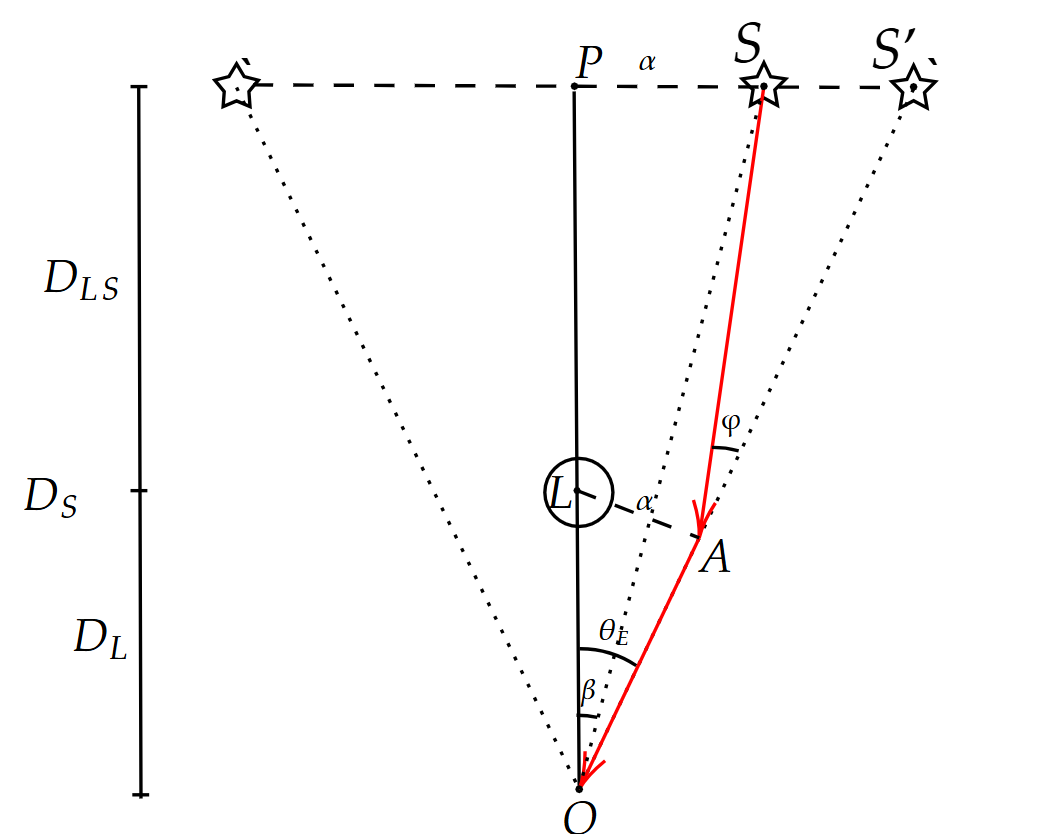
\includegraphics[width=0.9\linewidth]{imagens/anelE.png}
        \caption{Esquema da lente gravitacional}
    \end{figure}
    No esquema, o ponto \(O\) representa o observador, \(L\) o corpo massivo que atua como uma lente, \(S\) a posição real do objeto observado e \(S'\) sua posição aparente, \(\alpha\) é o parâmetro de impacto, \(\beta\) a separação angular entre o corpo observado e a lente, \(\theta_E\) o raio angular do anel de Einstein, \(\varphi\) o desvio angular causado por um corpo massivo. A distância \(\overline{OL}\) vale \(D_L\) e a distância \(\overline{OP}\) vale \(D_S\), de modo que \(D_S-D_L = D_{LS}\).

    Todos os ângulos são muito pequenos, de modo que \(\sin x \approx \tan x \approx x\). Além disso, por estarem no infinito, as retas \(\overline{OP}\), \(\overline{OS}\) e \(\overline{OS'}\) podem ser aproximadas como paralelas.

    É um resultado conhecido da Teoria da Relatividade Geral que o desvio da luz causado por um corpo massivo é dado por:
    \[\varphi = \frac{4GM}{\alpha c^2}\]
    \begin{alternativas}
        \item No limite em que \(\lim_{\alpha \rightarrow 0}\), encontre uma expressão para \(\theta_E\) em função das demais distâncias e ângulos fornecidos.
    
        \item O telescópio JWST obtém imagens no infravermelho, de comprimento de onda \(\lambda_{IV}\). Quão grande deve ser seu diâmetro para que ele possa resolver um anel de Einstein?
    \end{alternativas}

    
\end{pproblem}

\pts{4}
\begin{pproblem}
    Neste exercício, vamos estudar propriedades da excentricidade das órbitas e entender como ela se relaciona com a energia e o momento angular. Denotando \(\mu = GM\) e \(h=L/m\), faça o que se pede nos itens a seguir.
    \begin{center}
        \textbf{Parte I: O vetor excentricidade}
    \end{center}
    \begin{alternativas}
        \item Escreva uma expressão para a segunda lei de Newton no formato vetorial para um corpo de massa \(m\) orbitando um corpo de massa \(M\) a uma distância \(r\).
        
        \item Faça o produto vetorial da sua expressão por \(\mathbf{h}\) e prove que:
        
        \[\frac{d}{dt}(\dot{\mathbf{r}}\times \mathbf{h}) = \frac{\mu}{r}\mathbf{v} - \frac{\mu \dot{r}}{r^2}\mathbf{r}\]

        Onde \(\dot{\mathbf{r}}\) representa a velocidade radial e \(\mathbf{v}\) a velocidade.

        \item Podemos escrever o lado direito da equação anterior como:
        \[\frac{d}{dt}\left(A\mathbf{r}\right)\]

        Encontre o valor de \(A\).

        \item Integre os dois lados da igualdade encontrada e faça a multiplicação escalar de ambos os lados por \(\mathbf{r}\). Após isso, resolva para \(r\). O seu resultado deve ser bem parecido com o previsto somente pela geometria:
        \[r = \frac{p}{1+e\cos\theta}\]

        Encontre os valores de \(p\) e \(e\). \textbf{Não esqueça da constante de integração. Suas respostas podem depender dela.}

        \item No item anterior, \(e\) é a excentricidade da órbita. Voltando à equação obtida inicialmente no item \(c\), após a integração, ache uma forma de expressar \(\mathbf{e}\), como sendo um vetor de módulo \(e\) e que aponta diretamente para o corpo orbitado.
        
        \item Prove que a relação encontrada no item anterior pode ser escrita como:
        \[\mu \mathbf{e} = (v^2-\frac{\mu}{r})\mathbf{r} - (\mathbf{r}\cdot\mathbf{v})\mathbf{v}\]

        Para onde esse vetor aponta?
    \end{alternativas}
    \begin{center}
        \textbf{Parte II: Determinando elementos orbitais a partir do vetor excentricidade}     
    \end{center}
    Vamos definir o nosso sistema de coordenadas da seguinte maneira. Considere um sistema de mão direita, orientado de tal forma que o plano \(xy\) coincida com o plano equatorial e com \(\mathbf{z}\) apontando para o polo norte. Definindo o vetor nodal como \(\mathbf{n} = \mathbf{z} \times \mathbf{h}\).
    \begin{alternativas}
        \item Encontre uma expressão para \(\mathbf{h}\) em função das componentes do vetor \(\mathbf{r}\) e do vetor \(\mathbf{v}\). Após isso, encontre o vetor \(\mathbf{n}\) em função das componentes de \(\mathbf{h}\).

        \item Desenhe uma esfera celeste e represente nela: o plano do equador e uma órbita qualquer (que tenha inclinação diferente de 0). Nela, marque os seguintes ângulos: \(i\), a inclinação orbital, \(\Omega\) a longitude do nodo ascendente, \(\omega\) o argumento do periastro e \(\theta\), a anomalia verdadeira. 

        \item Encontre expressões para todos esses ângulos em função de \(\mathbf{e}\), \(\mathbf{h}\), \(\mathbf{n}\), \(\mathbf{r}\) e qualquer um dos vetores definidos no nosso sistema de coordenadas \(xyz\).
    \end{alternativas}

   
\end{pproblem}

\pts{5}
\begin{pproblem}\(\star\star\star\) (Adaptado IPhO 2018) Um dos efeitos mais interessantes da relatividade geral é a emissão de ondas gravitacionais (OG's) por binárias próximas. Um dos efeitos disso é a perda de energia do sistema. Nesta questão, iremos estudar esse efeito a fundo.

\begin{alternativas}
    \item Considere um sistema formado pelas estrelas 1 e 2, com massas \(M_i\) e distando \(r_i\) do centro de massa. Utilizando a segunda lei de Newton, é possível demonstrar que:
    \[\mathbf{a_1} = -\alpha \frac{\mathbf{r_1}}{r_1^n}\]
    Onde \(\mathbf{a_1}\) é o vetor aceleração da estrela 1. Encontre o valor de \(\alpha = \alpha (G, M_1, M_2)\) (lê-se \(\alpha\) em função de \(G, M_1, M_2\)) e de \(n\).

    \item A energia total do sistema binário pode ser expressa como:
    \[E = A(\omega, \mu, L) - \frac{GM\mu}{L}\]

    Onde \(\mu\) é a massa reduzida do sistema, \(M = M_1+M_2\) e \(L = r_1+r_2\). Encontre o valor de \(A\).

    \item A expressão anterior pode ser simplificada para:
    \[E = \frac{\beta GM\mu}{L}\]

    Onde \(\beta\) é uma constante adimensional. Encontre seu valor.

    A teoria correta da gravidade, a Relatividade Geral, foi formulada por Einstein em 1915 e prevê que a gravidade se propaga à velocidade da luz. Os mensageiros que carregam informações sobre a interação são chamados de ondas gravitacionais (OGs). OGs são emitidas sempre que massas são aceleradas, fazendo com que o sistema de massas perca energia.

    Considere um sistema de duas partículas pontuais, isoladas do restante do Universo. Einstein provou que, para velocidades suficientemente pequenas, as ondas emitidas: 1) têm uma frequência que é duas vezes maior do que a frequência orbital; 2) podem ser caracterizadas por uma luminosidade, ou seja, um poder emitido \(\mathcal{P}\), que é dominado pela fórmula:

    \[
    \mathcal{P} = \frac{G}{5c^5} \sum_{i=1}^3 \sum_{j=1}^3 \left( \frac{d^3 Q_{ij}}{dt^3} \right) \left( \frac{d^3 Q_{ij}}{dt^3} \right).
    \]

    Aqui, \( c \) é a velocidade da luz \( c \simeq 3 \times 10^8 \, \mathrm{m/s} \). Para um sistema de duas partículas pontuais orbitando no plano \( x-y \), \( Q_{ij} \) é a seguinte tabela (\( i, j \) indicam o número da linha/coluna):

    Os componentes de \( Q_{ij} \) são dados por:

    \[
    Q_{11} = \sum_{A=1}^2 \frac{M_A}{3} \left( 2x_A^2 - y_A^2 \right),
    \]

    \[
    Q_{22} = \sum_{A=1}^2 \frac{M_A}{3} \left( 2y_A^2 - x_A^2 \right),
    \]

    \[
    Q_{33} = -\sum_{A=1}^2 \frac{M_A}{3} \left( x_A^2 + y_A^2 \right),
    \]

    \[
    Q_{12} = Q_{21} = \sum_{A=1}^2 M_A x_A y_A.
    \]

    E \(Q_{i,j} = 0\) para todas as outras possibilidades. Aqui, \(x_A, y_A\) são as posições da estrela \(A\), com \(A=1,\ 2\) em um plano cartesiano com o centro de massa na origem.

    \item Escreva as coordenadas (\(x_1, y_1\)) e (\(x_2, y_2\)) em função de \(r_1, r_2, \omega\) e \(t\), com \(t\) sendo o tempo percorrido desde algum ponto específico da órbita.
    
    \item Para calcular a potência dissipada, a fórmula possui uma soma quádrupla. Resolver essa expressão "na tora" é algo bem complicado e demorado. Porém, felizmente, há um jeito mais bonito e elegante de resolvê-la. Para isso, comece escrevendo \(Q_{i,j}\) como uma matriz 3x3, da seguinte forma:
    
    \[Q = A\left(\begin{matrix}
        a_{11} & a_{12} & a_{13} \\
        a_{21} & a_{22} & a_{23} \\
        a_{31} & a_{23} & a_{33} \\
    \end{matrix}\right)\]

    Encontre o coeficiente \(A = A(\mu, L)\) e complete a matriz \(Q\).

    \item Do item anterior, você deve obter:
    \[Q_{ii} = A(b_i + j_i\cos(k t)), \ \ \ Q_{ij}^{i\neq j}= A(p_{ij} \sin(kt)) \]

    Encontre os valores de \(b_i\), \(j_i\), \(p_{ij}\) e \(k\).

    \item Agora, você é capaz de resolver para \(\mathcal{P}\) de maneira mais fluida. A expressão pode ser simplificada para:
    \[\mathcal{P} = \xi \frac{G}{c^5}\mu^2L^4\omega^6\]
    Encontre o valor numérico de \(\xi\).

    \textbf{DICA: } O somatório duplo:

    \[\sum_{i=1}^N\sum_{j=1}^N (A_{ij})(A_{ij})\]

    Onde \(A\) é uma matriz \(N\times N\) pode ser simplificado para:

    \[\sum_{i=1}^N\sum_{j=1}^N A_{ij}^2\]

    Que representa a soma quadrática de todos os elementos da matriz \(A\).

    \item Caso não houvesse a emissão de OG's, o sistema continuaria em equilíbrio indeterminadamente, mas devido à sua emissão, a energia do sistema não é conservada, fazendo com que haja uma variação na velocidade angular do sistema, \(\omega\). A fórmula para a variação temporal de \(\omega\) tem a seguinte cara:
    \[\left(\frac{d\omega}{dt}\right)^3 = (3\xi )^3 \frac{\omega^{11}}{c^{15}}(GM_C)^5\]
    
    Onde \(M_c\) é a chamada Massa \textit{Chirp} e \(M_c = M_c(M, \mu)\). Encontre uma fórmula para \(M_c\).

    \item Usando as informações obtidas acima, relacione a velocidade angular orbital \(\omega \) com a frequência das ondas gravitacionais \( f_{\text{OG}} \). Sabendo que, para qualquer função suave \( F(t) \) e \( a \neq 1 \):

    \[
    \frac{dF(t)}{dt} = \chi F(t)^a \implies F(t)^{1-a} = \chi (1-a)(t_0 - t),
    \]
    
    onde \( \chi \) é uma constante e \( t_0 \) é uma constante de integração, mostre que a equação do item anterior implica que a frequência das ondas gravitacionais é:
    
    \[
    f_{\text{OG}}^{-8/3} = 8\pi^{8/3} \xi \left( \frac{GM_c}{c^3} \right)^{(2/3)+p} (t_0 - t)^{2-p},
    \]
    
    e determine a constante \( p \).

    Em 14 de setembro de 2015, o evento GW150914 foi registrado pelos detectores LIGO, consistindo de dois braços em forma de L, cada um com 4 km de comprimento. Esses braços mudaram de comprimento relativo de acordo com a Figura abaixo. Os braços do detector respondem linearmente a uma onda gravitacional que passa, e o padrão de resposta imita a onda. Essa onda foi criada por dois buracos negros em órbitas quase circulares; a perda de energia por radiação gravitacional causou a contração da órbita e, eventualmente, a colisão dos buracos negros. O ponto de colisão corresponde, aproximadamente, ao pico do sinal após o ponto D, na Figura abaixo.

    \begin{figure}[H]
        \centering
        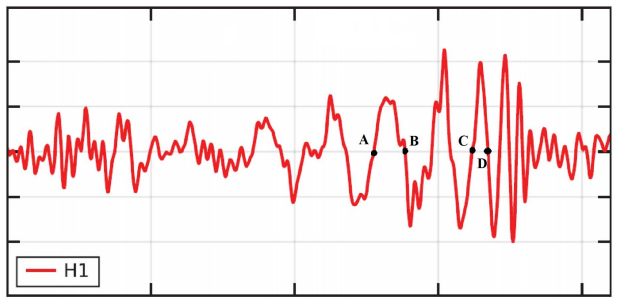
\includegraphics[width=0.7\linewidth]{imagens/grafico OG 1.png}
        \caption{Deformação, ou seja, variação relativa do tamanho de cada braço, no detector LIGO H1. O eixo horizontal representa o tempo, e os pontos A, B, C, D correspondem a \(t = 0,000\), \(0,009\), \(0,034\), \(0,040\) segundos, respectivamente.}
    \end{figure}

    \item A partir da figura, estime \( f_{OG}(t) \) em:

    \[
    t_{AB} = \frac{t_B + t_A}{2} \quad \text{e} \quad t_{CD} = \frac{t_D + t_C}{2}.
    \]
    
    Assumindo que a equação para \(f_{OG}\) é válida até a colisão (o que, estritamente falando, não é verdade) e que os dois objetos possuem massas iguais, estime a massa "chirp", \( M_c \), e a massa total do sistema, em termos de massas solares \( M_\odot \simeq 2 \times 10^{30} \, \text{kg}\).

    \item Estime a separação orbital mínima entre os dois objetos em \( t_{CD} \). 
    Assim, estime um tamanho máximo para cada objeto, \( R_{\text{max}} \). 
    Obtenha \( \frac{R_\odot}{R_{\text{max}}} \) para comparar esse tamanho com o raio do nosso Sol, \( R_\odot \simeq 7 \times 10^5 \, \text{km} \). 
    Estime também sua velocidade orbital linear no mesmo instante, \( v_{\text{col}} \), comparando-a com a velocidade da luz, \( \frac{v_{\text{col}}}{c} \).
\end{alternativas}


\end{pproblem}

\pts{3}
\begin{pproblem}(Barra 2024) Durante sua estadia no Hotel Fazenda Ribeirão, Hugo observava a estrela Plo I com seu telescópio. Comparando o seu espectro com o de outras estrelas, ele descobre que Plo I é uma estrela de nêutrons e estima sua massa como sendo \( M_1 = 2M_{\odot} \). Ele também observa que Plo I possui variações senoidais em sua velocidade radial ao longo do tempo e conclui que Plo I deve fazer parte de um sistema binário com outro corpo celeste, Plo II. Observando a curva de velocidade de Plo I, Hugo também determina que Plo I possui uma órbita circular de período \( P \) e velocidade radial máxima \( K \). Porém, ele não sabe qual é a massa \( M_2 \) de Plo II e nem qual é a inclinação \( i \) do plano orbital do binário em relação ao plano do céu, representada na figura a seguir.

    \begin{figure}[H]
        \centering
        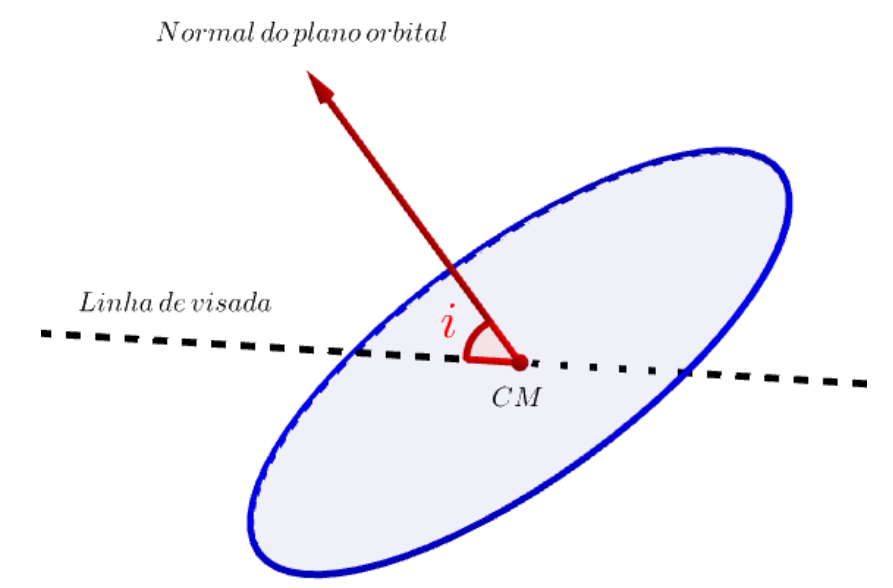
\includegraphics[width=0.8\linewidth]{imagens/figurabarra.png}
        \caption{Representação da órbita}
    \end{figure}

    \begin{alternativas}
        \item A partir da 3ª lei de Kepler e da 2ª lei de Newton, encontre uma expressão para a \textbf{função de massa} do sistema binário formado por Plo I e Plo II em termos de \( P \), \( K \) e constantes universais. Você pode utilizar que a função de massa é dada por:
        \[
            f = \frac{M_2^3 \sin^3 i}{(M_1 + M_2)^2}
        \]
    
        \item Utilizando suas medidas, Hugo calcula que a função de massa do binário é \( f = 46,2M_{\odot} \). Desejamos encontrar o valor mínimo \( M_{2,\text{min}} \) para a massa de Plo II, sabendo que ele corresponde ao caso em que \( i = 90^\circ \). Suponha \( M_{2,\text{min}} > M_1 \). A partir disso, determine \( M_{2,\text{min}} \). Seu resultado é condizente com a hipótese? Responda SIM ou NÃO, justificando com cálculos.
        
        \item Com base em sua resposta do item anterior, conclua: é mais provável que Plo II seja um exoplaneta, uma anã branca, uma estrela de nêutrons ou um buraco negro?
    \end{alternativas}

\pts{3}
\begin{pproblem} Juventino está localizado na sua base (não tão) secreta no Polo Norte terrestere. Após uma chama de emergencia de deduardo letodo, o mesmo precisa mandar um missél para o equador, afim de explodir a base de seu arqui inimigo: Raposo. 
    \begin{alternativas}
        \item Junvetino não está na sua melhor forma, e com toda a sua força, ele só consegue arremessar o foguete na primeira velocidade cósmica (a velocidade orbital para corpos próximos da superfície terrestre). Nessas condições, qual é o semi eixo da órbita do foguete lançado por Juventino?
        \item Qual a maior altura que o foguete chega?
        \item Qual o intervalo de tempo entre o Juventino lançar o foguete e a base de Raposo ser explodida?
    \end{alternativas}
    
\end{pproblem}
    
    
    
\end{pproblem}

\end{document}